
\section{Resolución}

\subsection{Desarrollo y proceso completo}

Para el desarrollo del proyecto, se ha optado por utilizar la metodología KDD (Knowledge Discovery in Databases) debido a su eficacia en proyectos de análisis y clasificación de datos. KDD proporciona una serie de pasos estructurados que abarcan desde la identificación de los datos hasta la implementación de modelos predictivos, esto es clave para manejar de forma eficaz la complejidad de nuestros datos de audio y garantizar una gestión coherente y organizada de todo el proyecto. Además, KDD ofrece un enfoque iterativo que nos permite ajustar y mejorar continuamente nuestros modelos a medida que avanzamos en el análisis de los datos.  

En cada una de las cinco etapas de la metodología KDD, se llevan a cabo procesos específicos para avanzar en el análisis y la clasificación de los datos de audio. La primera etapa, denominada ``database'', se centra en la identificación y selección de los datos relevantes para nuestro análisis. Luego, en la etapa de ``preprocesamiento'', se realizan diversas operaciones, para preparar los datos de manera óptima para su análisis posterior. 

La siguiente etapa es el ``entrenamiento'', donde se desarrollan y ajustan los modelos de clasificación de sonidos utilizando técnicas de aprendizaje automático. Posteriormente, en la etapa de ``comparativa de modelos'', se evalúan y comparan los diferentes modelos desarrollados para identificar el más adecuado para nuestro propósito. Finalmente, en la etapa de ``implementación'', se llevan los modelos seleccionados a entornos prácticos, lo que nos permite utilizar los resultados obtenidos en situaciones del mundo real.

\subsubsection{Database}

Comenzando por la parte de database, se realizó un análisis inicial de los datos disponibles. Se procesaron un total de 2,66 GB de datos, que consistían en 21,024 fragmentos de audio con diferentes tipos de sonidos no verbales de longitud variable. Sin embargo, durante este proceso se realizó una limpieza de los datos para eliminar fragmentos de audio con longitudes similares a 0, lo que resultó en un conjunto final de 20,502 audios para su análisis 

\subsubsection{Preprocesamiento}

En cuanto al preprocesamiento de los datos, se llevaron a cabo varias etapas importantes. En primer lugar, se realizó la normalización de los archivos de audio en formato ``.wav'', transformándolos en tensores de valores decimales. Además, se asignaron etiquetas en formato one-hot a los nombres de los archivos para facilitar su procesamiento y clasificación.

Posteriormente, se llevo a cabo la estandarización de las señales de audio para igualar las longitudes de los tensores de señal. Esto se logró mediante dos técnicas principales: el padding, que consiste en agregar valores nulos a los extremos de los tensores para igualar su longitud, y el random cropping, que recorta aleatoriamente fragmentos de los tensores para ajustar su longitud.

Además, se exploraron diversas técnicas para el procesamiento y análisis de datos de audio. Inicialmente, se optó por aplicar la transformada de Fourier a los fragmentos de audio. Esta técnica permitió descomponer las señales de audio en sus componentes de frecuencia, lo que resultó útil para identificar las características espectrales distintivas de diferentes tipos de sonidos. Sin embargo, conforme se avanzaba en el proyecto, se observaron limitaciones en términos de optimización y eficacia en la clasificación de sonidos al aplicar exclusivamente la transformada de Fourier. 


\begin{center}
    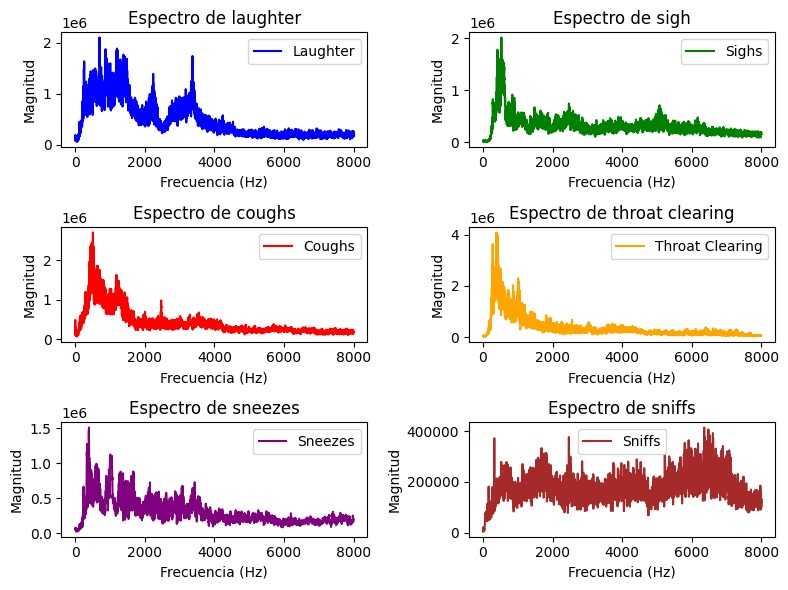
\includegraphics[width=0.5\textwidth]{ImagenesLatex/fourier.jpg}
\end{center}


Por lo tanto, se decidió explorar otras técnicas y se investigó Mel-frequency cepstral coefficients (MFCCs).
Los Mel-frequency cepstral coefficients (MFCC) son una técnica comúnmente usada en el procesamiento de señales de audio para extraer características importantes que describen la estructura espectral de una señal sonora. Esta técnica se basa en la idea de que el sistema auditivo humano no percibe todas las frecuencias de manera uniforme, sino que es más sensible a ciertos rangos de frecuencia, lo que se conoce como la escala de Mel.


\begin{center}
    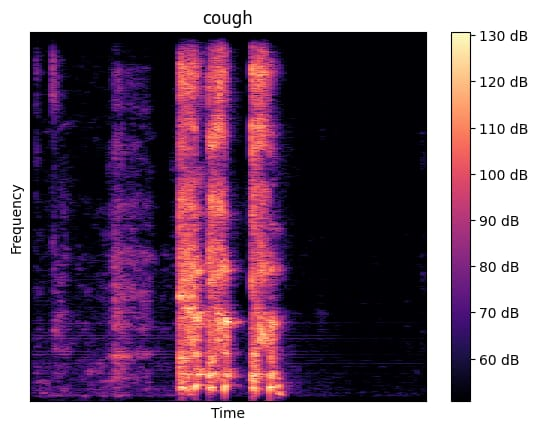
\includegraphics[width=0.5\textwidth]{ImagenesLatex/espectrograma.jpg}
\end{center}


No obstante, se continuó en la búsqueda por la mejor estrategia de procesamiento de datos. Después de implementar los MFCCs, se buscó la opinión de un consultor ingeniero externo. Este paso resultó crucial, ya que se proporcionó una perspectiva experta sobre cómo optimizar el enfoque. Tras consultar al ingeniero externo, se llegó a la conclusión de que la estrategia más eficiente sería implementar los algoritmos directamente sobre los datos originales de audio, aprovechando su estructura matricial, por lo que se descartó el uso de la transformada de Fourier y de los MFCCs. Esta recomendación permitió optimizar el proceso de procesamiento de datos y la aplicación de los algoritmos de manera más directa y efectiva.

En última instancia, dada la magnitud del conjunto de datos y la necesidad de administrar eficientemente la memoria y la capacidad de cómputo, se optó por implementar un input pipeline utilizando herramientas y pipelines de TensorFlow. Esta implementación permitió convertir los archivos de audio en tensores de valores decimales y organizarlos en lotes para su procesamiento por lotes. Esta modificación permitió continuar con el estudio del clasificador, ya que se estaban encontrando múltiples problemas debido a que la memoria de Google.Collab no era suficiente y se estaba imposibilitando el trabajo.

Esta conversión a tensores es fundamental ya que facilita el manejo de los datos en memoria y permite realizar operaciones matemáticas eficientes en ellos. Además, al utilizar tensores en lugar de datos de audio brutos, se redujo significativamente el consumo de memoria, lo que evitó errores de memoria y optimizó el rendimiento del sistema durante el procesamiento de los datos.  El input pipeline también permitió organizar los datos en lotes, lo que facilitó su procesamiento por lotes durante el entrenamiento de modelos de aprendizaje automático. Esto aceleró el proceso de entrenamiento y mejoró la eficiencia del sistema en general. 

\subsubsection{Entrenamiento}
En esta fase del KDD, se eligieron y entrenaron diferentes modelos matemáticos para el análisis del set de datos. El objetivo del proyecto es conseguir predecir las etiquetas de las señales de sonidos no verbales, para ello se entrenaron los siguientes modelos:
\begin{itemize}
    \item K-vecinos más cercanos (KNN)
    \item Redes de neuronas artificiales secuenciales (SNN)
\end{itemize}
Ambos algoritmos son supervisados, para la clasificación de datos nuevos se entrena al modelo con datos etiquetados y el modelo aprende en función de si ha clasificado bien o mal datos etiquetados.

La idea básica detrás de KNN es que los puntos de datos similares tienden a agruparse en el espacio de características. Cuando se clasifica un nuevo punto de datos (en este caso, un nuevo audio), el algoritmo busca los "K" puntos de datos más cercanos (vecinos) en el espacio de características. Luego, asigna la clase más común entre esos vecinos al punto de datos de prueba. Para KNN se obtuvieron resultados poco satisfactorios con precisiones inferiores al 50\%. Aunque es posible que se pudieran obtener mejores resultados, utilizando representaciones de los datos como espectrogramas basados en los coeficientes cepstrales de Mel, se tomó la decisión de abordar el problema de clasificación principalmente con redes neuronales artificiales.

Las redes neuronales en el contexto del aprendizaje automático (machine learning) son un tipo de modelo computacional inspirado en la estructura y el funcionamiento del cerebro humano. Están compuestas por unidades de procesamiento llamadas neuronas artificiales que están organizadas en capas y conectadas mediante conexiones ponderadas. Las redes neuronales articificiales o redes neuronales secuenciales (en adelante RNA), son excelentes en la clasificación de sonidos por ser capaces de aprender características complejas de los datos, su flexibilidad en la representación de datos y adaptabilidad, esto las convierte en clasificadores consistentes aprueba de fallos como pueden ser incompletitudes en los datos.

Se comenzó realizando arquitecturas secuenciales con capas densas. Las capas densas son un tipo de conexiones entre neuronas que conectan todas las neuronas de entrada con todas las de salida, y de manera automática utilizando regresores lineales ajustan mediante pesos como de importante es cada conexión. Este tipo de capas tienen la desventaja de que estudian de manera parcial el orden en el que aparecen los datos, y los sonidos que se pretenden estudiar tienen carácteristicas que son temporalmente dependientes, como puede ser tras una tos un sonido de inspiración o la variación en amplitud al final de la misma. Se probaron modelos más simples con pocas capas y más complejos con muchas capas. Los resultados fueron peores que los obtenidos con KNN y además el modelo se encontraba limitado por su arquitectura, no superando el umbral de 25\% a pesar de aumentar el número de capas.

Viendo los resultados anteriores, se probó con modelos basados en capas convolucionales unidimensionales, esta arquitectura permite a la red extraer información posicional de los eventos que ocurren en los audios, este tipo de capas utilizan múltiples filtros sobre ventanas de los vectores de amplitudes, obteniendo diferentes mapas de características. La finalidad de estas capas es reducir la dimensionalidad de los audios, llevando el espacio de dimensiones a otras más facilmente interpretables por regresores lineales.
La mejora al usar este tipo de modelos fue notable, tanto modelos sencillos como más complejos, el mejor modelo alcanzado en mayo de 2024 tuvo un precisión del 85\%, a continuación se muestra la tabla parámetros entrenables de la mejor arquitectura:
\begin{center}
    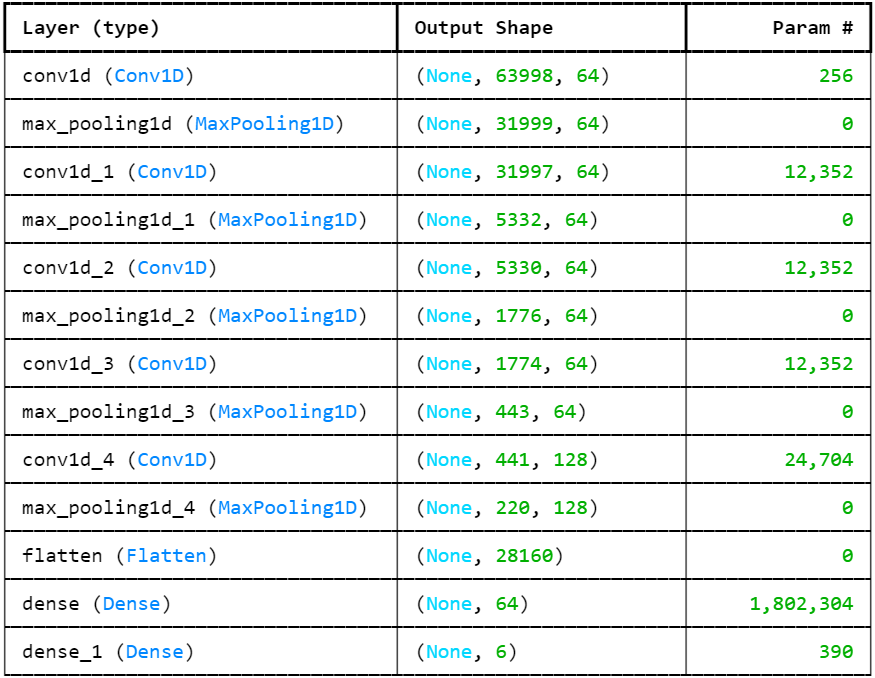
\includegraphics[width=0.8\textwidth]{ImagenesLatex/Conv1D_capas.PNG}
\end{center}
Los hiperparámetros principales para este modelo:

Una vez se definió la arquitectura se estimaron los hiperparámetros para cada modelo, se utilizaron para todos los modelos de RNA los siguientes:
\begin{itemize}
    \item Train(\%), Test(\%): 80\%, 20\%
    \item Batch size: 128 (máximo permitido por colab)
    \item Learning rate: Variable entre 0.01 y 0.001
    \item Epochs: dependiente del modelo
\end{itemize}
Para el mejor modelo el número de épocas fue 12.
\subsubsection{Comparativa de modelos}
Por simplicidad para la comparativa de modelos se tuvo en cuenta principalmente su precisión para resolver el problema en cuestión, se deja como trabajo a futuro el estudio en escalabilidad y ocupación en memoria de los parámetros entrenados.

Para la elección del modelo que se usará para la implementación real, se compararon los siguientes resultados:
\begin{center}
    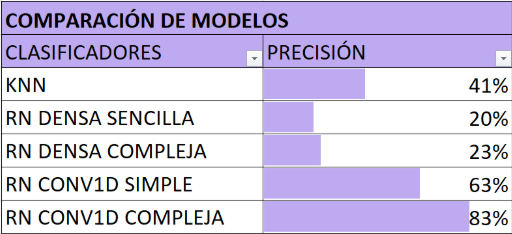
\includegraphics[width=0.8\textwidth]{ImagenesLatex/ComparacionModelos.PNG}
\end{center}

El mejor modelo obtenido en abril de 2024 fue el realizado con capas convolucionales 1D, que por tener más de 2 capas entra en la categoría de deep learning.

\subsubsection{Implementación}
Para la implementación del proyecto, se ha desarrollado una aplicación que ofrece una solución práctica para la detección en tiempo real de varios tipos de sonidos, como tos, aclaración de garganta, risas, suspiros, esnifar y estornudos.

La aplicación se inicia importando los módulos necesarios y configurando la detección de los tipos de sonidos, además de cargar un modelo previamente entrenado con una efectividad del 85\%. Luego, utiliza Matplotlib para mostrar las formas de onda de audio en tiempo real y capturar las muestras entrantes para su procesamiento. Mediante una función definida, la aplicación detecta los diferentes tipos de sonidos utilizando el modelo cargado y los presenta en un gráfico para una fácil comprensión.

El flujo de audio se inicia mediante SoundDevice y se crea una animación continua para visualizar de manera fluida las muestras de audio y sus clasificaciones. Esta implementación puede ser muy útil en diversos ámbitos profesionales, como en las llamadas telefónicas (para evaluar el nivel de satisfacción del cliente durante la llamada) y en servicios sanitarios (para supervisar el bienestar del paciente).